% v0.1
\chapter{Data retrieval and preprocessing}
In this chapter we will present parts of our pipeline intended for data retrieval and preprocessing.
Since we used a considerable amount of third party libraries and tools, we will explain them in detail and we will clarify our reasons for using them.
We will also provide some basic statistics of the data retrieved.

\section{Pipeline overview}
Our pipeline consists of python scripts and publicly available bioinformatics software.
When writing the code, we have taken care of its readability, sustainability and extensibility.

We implemented our pipeline in  workflow management system \emph{Snakemake} that was primarily designed for writing reproducible bioinformatics pipelines.
Snakemake is inspired by GNU make, but it uses python-like syntax with elements similar to pseudo code.
Furthermore, it is fully portable, depending only on Python executables and libraries.
Snakefile consists of rules, where each rule is defined by its input files, output files and shell commands.

When the Snakemake is executed, it runs first rule in specified Snakefile.
If the rule is missing input files, it scans through the whole Snakefile and looks for rules that are capable of creating required files.
This process is repeated until there is a rule which can be completed or until there is a rule whose input is not possible to create by any other rule.
In the former case the execution starts running, in the latter case an error message is displayed.
By this approach it is ensured that we do not execute any unnecessary rules nor any rules that have been already completed.
This is an important feature for our program as some rules can take several hours to complete, even on powerful computational cluster.
Another useful characteristic of the Snakemake engine is the ability to produce graphical visualization of particular Snakefile in format of directed acyclic graph.
Simplified graphical representation of our pipeline is in the Figure \ref{fig:dag}.

The pipeline starts with downloading of publicly available data.
After downloading, we merge all records and eliminate duplicated records.
Next, we extract genes of the bacteriophages.
Consequently, phage genomes represented as sets of genes are split into a training and a testing set.
Similarity between the genes from the training set are calculated and based on those, clusters of similar genes are produced.
From these clusters, the binary matrix is created.
This matrix is later used in classification.

\begin{figure}[h]
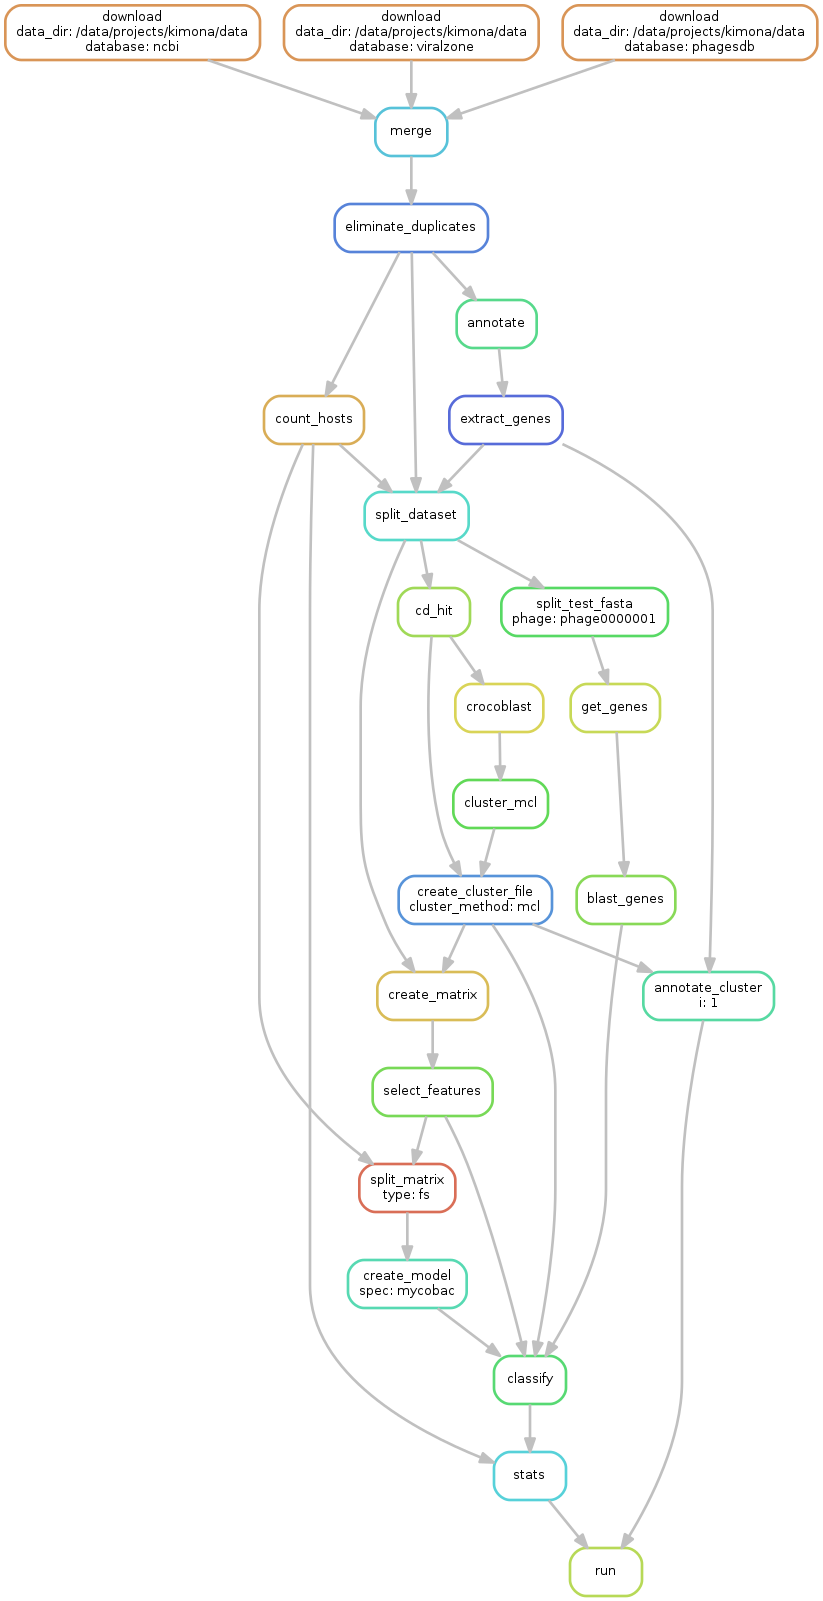
\includegraphics[height=\textheight]{./images/mcl.png}
\centering
\caption{Workflow visualization}
\label{fig:dag}
\end{figure}

\section{Downloading phage genomes}
The first step in our pipeline is downloading of data from three publicly available databases.
Although they cover the majority of currently sequenced and published phages, we made this step easily extensible for adding new sources of information in the future.
New sources can be added by writing a new download script, naming it \verb|{script_dir}\download_from_{db}.py| and appending this name into a variable \verb|DATABASES| in Snakefile.

\subsection{GenBank database}
National Center for Biotechnology Information (NCBI) provides an access to \emph{GenBank}\cite{genbank} database.
This database is a comprehensive source of genomic data with more than 200 million genomic sequences of all life’s domains.
NCBI administers the GenBank database free of charge and give researchers the possibility to access data through various interfaces as web-based retrieval services, FTP and Entrez\cite{entrez}.
Despite of these facts, there are shortcomings of using GenBank.
In the time of Next Generation Sequencing the amount of data flowing into GenBank database every day is enormous.
Therefore, it is unreasonable to check all the data.
Sequences are primarily submitted by individuals from all around the globe and are not thouroughly reviewed.
This causes redundancy of sequences and sometimes it even creates contradictions between information in system.

We obtained data using python library Biopython \cite{biopython}, which implements python wrapper NCBI Entrez.
Besides that, we used Biopython to facilitate  processing of standard file formats used in bioinformatics.
When downloading sequences, we also created unique identifiers for each record.
Those were used later in the pipeline.
Reasons behind the decision to use custom identifiers was the ability to remove duplicated sequences and the possibility to find out multiple sources of each sequence in our dataset.
Downloading from GenBank was our largest source of data with 6704 downloaded records.

\subsection{ViralZone database}
ViralZone provides highly reliable data about viruses, including bacteriophages.
Information about the structure of a capsid, a genome, life cycle, replication mechanisms, taxonomy, geographical location and host are included.
This website does not store sequences internally, rather it delivers links to \emph{RefSeq}\cite{refseq} database.
Compared to GenBank, RefSeq database contains fewer sequences, but all of these sequences are curated and manually reviewed.

Our custom script was used to download records from RefSeq database.
Although, large portion of sequences downloaded was identical with GenBank records, some sequences were unique.
Another advantage in performing this action was that it enabled us to pair genomic sequences from RefSeq with more comprehensive information from ViralZone portal.
By performing this process, we obtained 2107 records.

% end of session 2018.04.18
% wc chapter* = 32521 letters

\subsection{PhagesDB}
\emph{PhagesDB} is a database specialized in bacteriophages infecting bacteria from phylum Actinobacteria.
This phylum is of great importance, because of its contribution to the soil system.
This phylum also contains the genus Mycobacterium, which includes pathogens causing tuberculosis and leprosy in humans.
The database was designed to avoid the time between sequencing and data availability.
Authors declare, at the time of their publication, there was more than 600 records of bacteriophages that were not yet in GenBank.
Furthermore, PhagesDB stores more biologically relevant data , such as discovery details, sequencing details, characterization details, sequence file and a plaque picture.
We downloaded 2491 phage records with our automatized script using the publicly available Application Programming Interface (API).

\subsection{Merging and removing of duplicated records}
Downloaded records were  highly redundant, mainly because many of those records were present in  more databases at once.
To solve this issue, we merged datasets together and removed duplicated records.
For merging we used the standard unix command \verb|cat|.
For removing duplicated sequences, we created a custom Python script.
This script made use of custom identifiers, which were assigned to every sequence that was downloaded.
In case more identical sequences were found, their identifiers were rewritten with the identifier of the first sequence.
This approach preserved the relationships between one particular sequence and all data related to it.
Thus, we were able to track phages, based on their identifiers, to their source databases and also connect them with all data that was already downloaded.
After removing of duplicated sequences our dataset contained 6277 phage records.

\section{Extraction and annotation of genes}
Next step in the pipeline was to identify genes on genomic sequences and annotate them with their biological function.
Although gene annotations of particular genomes are part of genomic records in used databases, we decided to annotate sequences from scratch.
This way we ensured consistency of annotations accross our data .
Another advantage of annotating from scratch is that annotations will always be up-to-date with current human knowledge.

\subsection{Prokka}
We used publicly available pipeline called \emph{Prokka} \cite{prokka} to identify and annotate genes.
First, coordinates of coding DNA sequences (CDS) were found with Prodigal tool\cite{prodigal}.
CDSs are regions of genome that almost always start with AUG codon and end with a stop codon.
These regions can be directly translated into amino acid chains using standard codon table.
After the locations of genes are predicted, Prokka can start to annotate functions of all CDSs.
This is usually done through comparing of a sequence to a database of sequences with an experimentally determined function.
The function of protein with the best match is then assigned to the new CDS.
Prokka, by using this approach searches through multiple databases.
Starting with the most reliable source, which is usually the smallest, it scans all the databases, continuing with the less accurate one.
The databases used with their corresponding order are as follows:
An optional user-defined database, UniProt\cite{uniprot}, RefSeq\cite{refseq}, Pfam\cite{pfam} and TIGRFAM\cite{tigrfam}.
If no match is found across databases, protein is labelled as \verb|hypothetical protein|.

% end of session 2018.04.12
% wc chapter* = 33657 letters

\subsubsection{UniProt}
The UniProt database is acollection of more than 60 million protein sequences and their corresponding detailed information.
Prokka uses just a small fraction of proteins backed up by experimental evidences.
This typically provides information about approximately 50\% of queried proteins.

\subsubsection{RefSeq}
RefSeq, provides information about genomic and protein sequences.
It contains more than 2.5 million protein records.
Multiple sources are integrated in annotation of genes.
Furthermore, all records are curated by the NCBI staff members.

\subsubsection{Pfam}
Pfam is a database consisting of protein families and domain records.
Protein families are groups of protein sharing evolutionary history.
This shared evolutionary history is often expressed by closely related functions and sequence similarity.
Protein domains are parts of a protein sequence responsible for a particular interaction. 
Members of the same protein domain usually share a high sequence similarity.
Protein families and domains are mostly characterized by Profile Hidden Markov Models.
Pfam incorporates more than 6100 of those models.

\subsubsection{TIGRFAM}
TIGRFAM, similarly as Pfam, contains protein families characterized by Profile Hidden Markov Models.
It contains more than 4200 models with comprehensive description of family structure and function.

\vspace{\baselineskip}

All of the aforementioned databases are regularly updated, which guarantees the most up-to-data annotations.
After annotation, resulting genes were selected and saved to files in format suitable for further use in the pipeline.

\section{Datasets used}
At the beginning of this step, our dataset consisted of: phage genomic records, their corresponding genes, information about phage hosts and functional annotation of genes.
As our work used techniques of supervised machine learning, we needed to split the dataset to a \emph{training set} and a \emph{testing set}.
Furthermore, we created set for other records, which we decided not to use due to missing information about host or due to host outside of our group of interest.
We decided to group phages according to the genus of their hosts.
After calculating the number of phages in each group, we selected first eight genera with the highest count of records as groups of our interest.
These were Mycobacterium, Streptococcus, Escherichia, Gordonia, Arthrobacter, Pseudomonas, Lactococcus and Staphylococcus.
Number of phages within each group can be found in the Table (\ref{tab:counts}).
All other genera were excluded from the dataset due to the insufficient number of samples.
Phages without information about their hosts were also excluded.
Subsequently, we divided remaining data into a training set and a testing set at a ratio of 4:1.
The resulting training set included 2787 records of bacteriophages and resulting testing set included 699 records.

\begin{table}
 \centering
        \begin{tabular}{ l  r  l  r }
         \hline
         genera & count & genera & count \\
         \hline
         Mycobacterium & 1619 & Streptococcus & 354 \\
         Escherichia & 323 & Gordonia & 293 \\
         Arthrobacter & 240 & Pseudomonas & 236 \\
         Lactococcus & 219 & Staphylococcus & 184 \\
         \hline
        \end{tabular}
        \caption{Counts of records within genera}
        \label{tab:counts}
\end{table}

%--------deeply described parts-------------------------------------------------
% v0.1
\section{Sequence alignment}
In this section we would like to thoroughly explain what sequence alignment is, since it is one of the most essential tasks in bioinformatics.
We will describe two main types of sequence alignment, with emphasizing the differences.
We will also explain the basic algorithms used for solving these problems and we will also describe the heuristic method used in case the input is too big to be computable by standard approaches that guarantee optimal solution.
At the end of this section we will describe, how we used the algorithms in our analysis.

\subsection{Global alignment}
\subsubsection{Usage}
Global alignment is commonly used for comparison between two sequences with roughly the same length.
This comparison can help us to discover mutations in a sequence that causes a certain phenotype, or we can use the comparison to determine highly conserved regions with a potential to carry a gene.
The relationships between conserved regions and mutations in certain sequences often serve as a basic assumption for construction of phylogenetic trees.
Therefore, global alignment can tell us a lot about the nature of evolution.
Global alignment is also capable of calculating a similarity score for two sequences.

\subsubsection{Problem statement}
Let the input for the problem be a set of two sequences consisting of nucleotides, for example, $ X = ATTGATGG $ and $ Y = AATTCAAC $.
Then the output is represented as a matrix, where each row is one sequence with possible gaps between nucleotides.
We can see potential solutions in the Table (\ref{tab:potsol})

\begin{table}
  \centering
	\begin{tabular}{ l | r }
	\verb|A-TTGATGG| & \verb|-ATTG-ATGG| \\
	\verb|AATTCAAC-| & \verb|AATTCAAC--| \\
	\end{tabular}
  \caption{Global alignment examples}
  \label{tab:potsol}
\end{table}

As we can see, every alignment could have more than one valid solution.
Despite of multiple possible solutions, not every solution is of equal value to us.
We want to find the best possible solution to this problem and for this purpose, we implement a scoring scheme to determine what is the best solution.
Scoring scheme consists of rules, which add numerical value to each column of pairwise alignment.
For example, we can evaluate match in column with score $+1$, mismatch with score $-1$ and alignment to gap with score $-1$.
With this scoring scheme, we can evaluate quality of a particular alignment.
For alignment on the left side of the Table (\ref{tab:potsol}), resulting score is $+1-1+1+1-1+1-1-1-1 = -1$ and for alignment on the right side of the Table (\ref{tab:potsol}) $-1+1+1+1-1-1+1-1-1-1 = -2$.
From this example we can see that according to our scoring scheme, alignment on the left is better.

\subsubsection{Scoring schemes}
In practice, we could use a more complex scoring scheme that better reflects reality.
For example, substitution between purines (adenine, guanine) or substitution between pyrimidines (cytosine, thymine) occur more often, because they do not require change in the number of rings in the chemical structure of these nucleotides.
When we try to align two proteins, a more complex scoring scheme is inevitable.
Amino acids differ in many parameters such as: polarity, size and structure of their side chains.
This influences the probability of a substitution occurring between two amino acids.
Therefore, there is a higher probability that Leucine will be substituted for Isoleucine, rather than Aspartic Acid.
To solve the complexity of substitutions between amino acids, matrix BLOSUM62 (\ref{fig:blosum}) was created.
Another layer of complexity, that does a better job of reflecting reality is the affine gap penalty function.
This reflects the fact that insertions and deletions do not usually occur only on one nucleotide, but often a longer region of DNA is deleted or inserted.
Affine gap penalty solves this issue by having a higher negative score for opening a new gap in alignment and a lower negative gap for extension of an already created gap.

\begin{figure}[ht]
  \centering
	
\includegraphics[width=\textwidth]{./images/blosum62.png}
  \caption{BLOSUM62}
  \label{fig:blosum}
\end{figure}

% end of session 16.04.2018

\subsubsection{Needleman-Wunsch algorithm}
For searching optimal global alignment, we usually use the Needleman-Wunsch algorithm.
It is an algorithm from a group of dynamic programming algorithms.
This means that the main problem is divided into smaller problems, which are computable more easily and solutions to them are stored in memory.
At each occurrence of a small problem, we can look into stored solutions, where we can find it.
Then the main problem is reconstructed from already computed subproblems.
Dynamic programming algorithms offer saving time on computation at the expense of a higher memory usage.

\begin{figure}[ht]
  \centering
	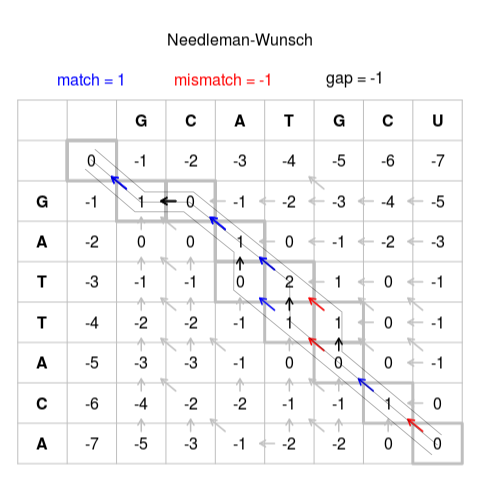
\includegraphics[width=\textwidth]{./images/needle_wunsch.png}
  \caption{Needleman-Wunsch}
  \label{fig:glal}
\end{figure}

Needleman-Wunsch algorithm produces a table as shown in the Figure (\ref{fig:glal}).
It starts by putting the first sequence we want to align to the first row and the second sequence to the first column.
Before each sequence there is one gap to cover the case if we would not want to align first letter of a particular sequence right from the beginning.
The table is then initialized with a series starting from 0 and decreasing by 1 each step on the second row and with the same series on the second column.
After initialization, the table starts to be filled from top left corner following this rule:\\
Into each cell $A_{i,j}$ write maximum of:
\begin{itemize}
\item $A_{i-1, j-1} + s()$,
\item $A_{i-1, j} + g()$,
\item $A_{i, j-1} + g()$,
\end{itemize}
where $s(X_i, Y_j)$ returns score of match/mismatch from scoring scheme and $g$ returns a score of the gap penalty (possibly affine gap).
The final score of the alignment can be found in the bottom right corner of the filled table.
Specific alignments can be found by tracking all possible paths to this value.
The time and space complexity of Needleman-Wunsch algorithm is $\mathcal{O}(nm)$, where $n$ is the length of the first sequence and $m$ is the length of the second sequence.

\subsection{Local alignment}
\subsubsection{Usage}
In comparison with global alignment, local alignment search for regions inside sequences with high similarities and does not provide alignment from beginning to end.
It is generally useful when searching for a small subsequence inside a vast sequence.
For example, searching for a gene inside the whole bacterial genome.
It can be also used when comparing two different sequences and we want to find out if they contain any highly similar sequence.

\subsubsection{Problem statement}
Similarly to what we have done with the global alignment, in this problem we search for optimal local alignment according to the defined scoring system.
The difference is that we do not know where the alignment in both sequences starts and where it ends.
For example, $ X = TAATAACTCTCTGAATAA $ and $ Y = CGGCGGCGGTCTCTGCC $ can be aligned as in the Figure (\ref{tab:loal}) and the score is calculated just from the first aligned base to the last aligned base.

\begin{table}
  \centering
	\begin{tabular}{ c }
	\verb|--TAATAACTCTCTGAATAA| \\
	\verb%     	|||||| 	% \\
	\verb|CGGCGGCGGTCTCTGCC---| \\
	\end{tabular}
  \caption{Local alignment example}
  \label{tab:loal}
\end{table}

\subsubsection{Scoring}
Scoring of local alignment is similar to global alignment and we are allowed to use the same methods we use in the global alignment.
Since the score is calculated just from the first aligned base to the last aligned base, the score of our local alignment would be $+1+1+1+1+1+1 = 6$, because there are 6 matches ($+1$) and no gaps ($-1$) or mismatches ($-1$).

\subsubsection{Smith-Waterman algorithm}
Local alignment can be found with dynamic programming algorithm similar to Needleman-Wunsch algorithm.
This is called Smith-Waterman algorithm and there are only two changes compared to Needleman-Wunsch.
First change is that matrix is not initialized with decreasing series, but second row and second column are filled with zeroes.
Second difference is in the rule as follows:\\
Into each cell $A_{i,j}$ write maximum of:
\begin{itemize}
\item $0$,
\item $A_{i-1, j-1} + s()$,
\item $A_{i-1, j} + g()$,
\item $A_{i, j-1} + g()$.
\end{itemize}
After completing the table, we need to find the highest number in it.
This number is a resulting score of our local alignment.
Following the path similarly as in global alignment we can reconstruct the alignment.
The space and time complexity of this algorithm is also $\mathcal{O}(nm)$.

% TODO: poriadne prerobit
\subsection{Word methods}
Needleman-Wunsch and Smith-Waterman algorithms are sufficient for simple comparisons of sequences, but their time complexity is not good enough when we want to search through very long sequences that are common in genomics.
It is often the case that we want to find the most similar sequence to ours in enormous bioinformatics database containing genomes of large amount of organisms.
This is particularly useful if we want to find the potential source of our sequence or comparing it to all known proteins to get some indicators about its potential function.
For this purpose, various heuristic algorithms were developed.
These algorithms do not guarantee finding the most optimal solution but are orders of magnitude faster and therefore usable also for searching in vast databases.

\subsubsection{BLAST}
%The basic algorithm consists of searching seeds from database on the query sequence and then extending those seeds into neighbouring bases.
%This approach provides orders of magnitude faster alignment method than classical Smith-Waterman algorithm \cite{smith_waterman} with comparable sensitivity.
Basic Local Alignment Search Tool (BLAST) \cite{blast} is probably the most widely used tool in bioinformatics.
The algorithm distinguishes between target sequences and query sequences.
Target sequences are sequences from which we create a database of all included k-mers.
For every k-mer in every sequence we save its position.
For example, for sequence GATCGATAG and given $k=3$ we create database as follows:
\begin{verbatim}
GAT = 1, 5
ATC = 2
TCG = 3
CGA = 4
ATA = 6
TAG = 7
\end{verbatim}
Next, we find every k-mer from query sequence in the database.
The matching k-mers are called cores of alignment and serves as starting points for extending of alignment.
The extending is performed in a similar manner to that of Smith-Waterman algorithm.
The difference is that we do not need to search through the whole matrix, but we search for good alignments only in the immediate surrounding of cores.
Firstly, we extend cores without the possibility to insert any gaps into alignment.
Secondly, we can join these extended cores together using the gaps, if the resulting score will be bigger than before joining.

\subsubsection{E-value}
E-value is used to assess the relevancy of the resulting alignment.
It can be interpreted as how many alignments in database could reach the same score or better purely by chance.
This means, the closer the E-value is to zero, the higher level of significance can be assumed.
E-value is automatically produced by BLAST.

\subsection{Alignment in the pipeline}
In our pipeline, we used alignment to find similarity scores between genes in the training set.
We needed these scores later in the pipeline at clustering step.
Software CrocoBLAST was used for this purpose.
CrocoBLAST is a wrapper around BLAST algorithm which makes better use of parallelization than standard BLAST maintained by NCBI.
With this software we were able to reduce the time needed for the alignment step from around four days to one day.
Resulting file was in tab separated format, where first column was gene identifier of query sequence, second column was gene identifier of the target sequence and third column was e-value of alignment.

\section{Data clustering}
In this section we will explain what we mean by data clustering and how we used it in our program.
We will describe three approaches we tried and we will describe two algorithms for clustering.

\subsection{Usage}
Data clustering is used to group data according to some similar characteristics.
In our case, we clustered genes with sequential similarities.
We expected those genes to have closely related functions.

\subsection{Definition of problem}
Clustering is a problem where we want to determine closely related entities and put them in distinct groups, also called clusters.

\subsection{Markov Cluster Algorithm}
\subsection{Spectral clustering}
\subsection{Clustering in our pipeline}
Clustering is a problem where we want to determine closely related entities and put them in distinct groups, also called clusters.
In order to be able to distinguish which entity is more closely related to another, we usually use similarity matrix.
To create a similarity matrix we used tab separated file described in previous section.
In this section we will mention different approaches we used for clustering. 
% http://www.paccanarolab.org/scps/
\subsection{Markov Cluster Algorithm}
First approach we used was Markov Cluster Algorithm. 
We used already implemented version called mcl \cite{mcl}.
This software is often used in bioinformatics for clustering of sequences based on their similarity.
It has the capability to determine number of resulting clusters automatically and except input data, it requires only one parameter.
This parameter is called inflation and usually takes float number values from 1.2 to 5.0.
Smaller values results in less and bigger clusters.
In our work we needed as few clusters as possible, mainly due to number of phage records in our dataset.
In case of too many clusters we would have too many features for classifier and we would risk overfitting of our final models to training dataset.
For these reasons we used inflation value 1.2, which created 15017 clusters.

\subsection{Markov Cluster Algorithm with global alignment}
To get more accurate clustering we tried different approach, where we determined similarity score of alignments with needleman-wunsch algorithm. \cite{needleman-wunsch}
This algorithm is able to calculate best global alignment score of given protein sequences.
The difference between global alignment and local alignment is that former aligns sequences from end to end.
The resulting score was then used as input to mcl algorithm described in previous section.
By this approach we created 9176 final clusters.

\subsection{Spectral clustering}
Spectral clustering is different algorithm used for clustering.
In this work we tried SCPS implementation\cite{scps}.
Authors of this bioinformatics software declare quality of clusters quantified by a measure that combines sensitivity and specificity to be better by 28\% in comparison to mcl algorithm.
Unfortunately, memory required by this program was too high and we were not able to run it on our server with all input data. 

%-------------------------------------------------------------------------------
%--------end of deeply described parts--------------------------------------
%-------------------------------------------------------------------------------
%--------end of deeply described parts------------------------------------------

\section{Annotation of gene clusters}
Clusters of genes were annotated to determine their function.
We expected proteins with similar biological function to be included in same cluster.
For functional annotation of particular proteins we used software \emph{InterProScan} \cite{interpro}.
This tool scans given protein sequences against the protein signatures in databases PROSITE \cite{prosite}, PRINTS \cite{prints}, Pfam \cite{pfam}, ProDom \cite{prodom} and SMART \cite{smart}.
After acquiring of annotations for all proteins in a particular cluster, we calculated number of occurrences of each distinct biological function.
These statistics represent our annotation of a certain cluster.
Our expectation of clusters containing proteins with similar function was met in most cases, although the information about particular proteins were sparse with a lot of proteins without any information.
Therefore, we assumed that reasonable clustering was achieved.

\section{Reducing phage genomes}
One of the most crucial part of our analysis was \emph{binary matrix} created in this step.
Rows in this matrix represented particular phage records and columns represented particular protein clusters.
The entry $a_{i,j}$ in matrix was filled with $1$ if phage $i$ contained gene from cluster $j$ and $0$ otherwise.
Custom python script and files produced in previous steps were used for this task.
Resulting matrix contained 2787 rows and 15017 columns and served as a main input file for the machine learning algorithms.